\documentclass[]{article}

\usepackage[dutch]{babel}
\usepackage{pgf-pie}
\usepackage{url}
\usepackage[utf8]{inputenc}
\usepackage[T1]{fontenc}
\usepackage{amsthm}
\usepackage{amsmath}
\usepackage{qtree}
\usepackage{footnote}
\theoremstyle{definition}
\newtheorem{ex}{Voorbeeld}[section]

\title{Natural Language processing for Knowledge Representation} \author{Jens
  Claes}

\newcommand{\example}[1]{\textit{``#1''}}

\begin{document}

\maketitle

%\section{Inleiding}
% TODO
% An introduction that explains the subject to the reader and gives an answer to the following questions:
    % What is the research question / problem of the thesis?
    % Why is it relevant?
    % What did others do to solve this problem and why is this not enough?
    % What do you do differently / what is new / what are the contributions of this work?
% Background
% Overview of related work
% Problem statement
% Planning (brief)

% TODO nalezen

\section{Inleiding}
\paragraph{} Vele bedrijfsprocessen worden geregeld door specificaties. Deze worden vaak geschreven in een natuurlijke taal, door een domein expert. Vervolgens worden deze specificaties vertaald naar uitvoerbare programma's. Bij deze vertaling sluipen er fouten in. Bovendien zijn er vaak meerdere programma's die elk opnieuw de specificatie moeten implementeren. Zo ontstaan er niet alleen inconsistenties met de specificatie, maar ook tussen de verschillende programma's onderling. Ten slotte is het moeilijk om de specificatie achteraf nog aan te passen omdat alle programma's dan aangepast moeten worden.

\paragraph{} Het antwoord van de academische wereld op deze problemen, is het \textit{Knowledge Base}-paradigma. In dit paradigma staat een kennisbank centraal. Deze kennisbank bevat de kennis over de wereld (i.e. de specificatie). Deze kennisbanken kunnen gebruikt worden in \textit{Knowledge Base Systems (KBS)}. Deze systemen bevatten een kennisbank en programma's die de kennisbank als invoer nemen en hier verschillende inferenties op doen. Om de kennis voor te stellen, kan men gebruik maken van een formele taal (zoals eerste-orde-logica). Zo'n talen hebben een eenduidige semantiek. Er is dus maar één mogelijke manier waarop de zin geïnterpreteerd kan worden. Dit in tegenstelling tot natuurlijke taal waar zelfs simpele zinnen al snel meerdere betekenissen kunnen hebben. In dit paradigma moet de specificatie in natuurlijke taal dus vertaald worden naar een vorm waar het KBS-systeem mee overweg kan: de formele specificatie. Deze specificatie wordt slechts eenmaal geschreven en vervolgens wordt ze gebruikt in alle programma's. Zo is het niet meer mogelijk dat de programma's onderling inconsistent zijn. Ze gebruiken namelijk allemaal dezelfde formele specificatie. Daardoor is ook het aanpassen van de specificatie makkelijker. Enkel de formele specificatie moet aangepast worden, de programma's blijven hetzelfde.

\paragraph{} Het probleem met deze aanpak is dat er nog steeds een vertaling moet gebeuren van natuurlijke taal naar een formele taal. De specificatie in natuurlijke taal wordt vaak opgesteld door een domein expert die niet vertrouwd is met formele talen. De formele specificatie wordt dan weer opgesteld door een KBS expert. Deze persoon kent formele talen maar heeft een beperkte kennis van het domein. Door deze mismatch van kennis, is de feedback loop tussen de twee experten beperkt. Het is dus nog steeds mogelijk dat er fouten sluipen in de vertaling.

\paragraph{} De vraag rijst dus of we een formele taal kunnen ontwerpen die toegankelijk is voor domein experten, rijk genoeg is voor praktische problemen en toepasbaar is binnen het KBS paradigma.

\paragraph{} Deze thesis onderzoekt of een formele natuurlijke taal het antwoord is op die vraag. Hieronder verstaan we (een subset van) een natuurlijke taal met een formele, eenduidige semantiek. Talen die een subset zijn van een natuurlijke taal worden ook wel gestructureerde natuurlijke talen of CNL's (naar het Engelse \textit{Constructed Natural Language}) genoemd. Deze talen verschillen van hun gasttaal doordat ze een aantal zinsconstructies niet toelaten. Dit kan bijvoorbeeld de leesbaarheid en consistentie van een taal verhogen. Voor ons zijn ze interessant omdat ambigue constructies op die manier verboden kunnen worden.

Naast constructieregels bevat een formele natuurlijke taal vaak ook interpretatieregels. Deze laatste bepalen hoe een ambigue zin in de nieuwe taal geïnterpreteerd moet worden. De moeilijkheid ligt erin om deze regels te beperken in aantal en in complexiteit.

Het grote voordeel van een formele natuurlijke taal is dat natuurlijke taal al gebruikt wordt bij het opstellen van de specificatie. Een voorbeeld van een domein waar specificaties een grote rol spelen is vereistenanalyse. Ook hier zien we dat specificaties vaak in natuurlijke taal worden opgesteld. Zo toont figuur \ref{fig:natural-language-use} het gebruik van natuurlijke taal in vereistenanalyse in 1999. Slechts 5 procent van de specificaties werd toen in een formele taal opgesteld. 16 procent werd zelfs al in een gestructureerde natuurlijke taal opgesteld, niet per se met een formele betekenis.

\begin{figure}
  \label{fig:natural-language-use}
  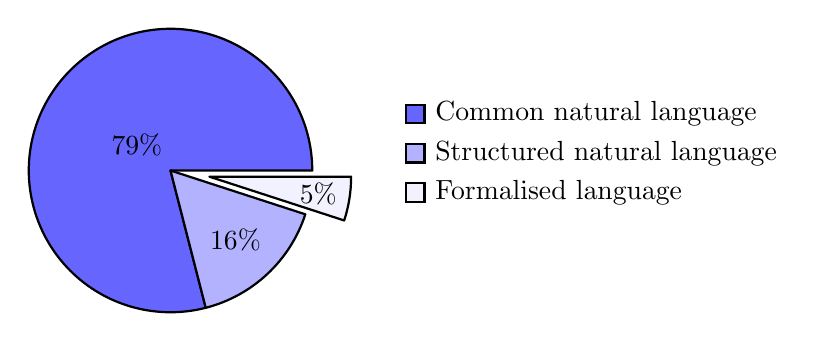
\begin{tikzpicture}
      \pie[text = legend, radius = 1.8, explode = {0, 0, 0.5}, color = {blue!60, blue!30, blue!5}]{79/Common natural language, 16/Structured natural language, 5/Formalised language}
  \end{tikzpicture}
  \caption{Gebruik van natuurlijke taal in vereistenanalyse in 1999 (van figuur 5 in \cite{Luisa2004})}
\end{figure}

\section{Achtergrond}
TODO

\section{Eerder werk}
In het verleden zijn er al meerdere CNL's gemaakt. Sommige zijn ontwerpen om de leesbaarheid van de specificaties te verhogen en hebben geen formele semantiek. Kuhn heeft een classificatieschema ontwerpen voor al deze CNL's \cite{Kuhn2014} genaamd PENS: Precision (hoe ambigu/formeel is de taal), Expressivity (welke problemen kunnen we uitdrukken), Naturalness (hoe vlot leest de taal), Simplicity (hoe simpel is de taal). In dezelfde paper lijst Kuhn ook een heleboel CNL's op met hun geschiedenis en nut alsook hun classificatie volgens het PENS-schema.

Meer in het algemeen is het omvormen van teksten in natuurlijke taal tot formele modellen al gebeurd in verschillende domeinen: in vereistenanalyse, in het paradigma van business rules, binnen de computationele linguïstiek en ten slotte in het domein van kennisrepresentatie. Deze sectie geeft een kort overzicht van wat er al gebeurd is in al deze domeinen. Voor een completer overzicht van CNL's, verwijzen we naar Kuhn \cite{Kuhn2014}.

\subsection{Vereistenanalyse}
\paragraph{Circe} De tool Circe \cite{Ambriola1997} wordt gebruikt in vereistenanalyse. De gebruiker moet een vocabularium, een set van substitutieregels en een specificatie in natuurlijke aanleveren. De tool probeert dan steeds de beste regel te vinden om zo de tekst geleidelijk aan te transformeren naar een formeel model. Het grote voordeel van de methode is dat er regelsets bestaan voor meerdere soorten modellen: data flow modellen, entity-relationship modellen, ...

Verder is het in Circe mogelijk om in het vocabularium woorden te taggen. De regels kunnen hier dan gebruik van maken om te bepalen of ze van toepassing zijn op bepaalde zinnen. Op die manier introduceert Circe types in het vocabularium.

Een voorbeeld (uit \cite{Ambriola1997}): \example{bron/UIT STUURT data/INFO NAAR doel/IN}. De woorden \example{stuurt} en \example{naar} liggen vast in de regelset. De andere 3 woorden komen uit het vocabularium. Deze moeten een bepaalde tag hebben om te matchen met de regel. Er zijn dus drie types in deze zin: entiteiten die informatie kunnen versturen, entiteiten die informatie kunnen ontvangen en informatie die verzonden kan worden.

Circe is geen CNL. Zinnen die niet matchen met een substitutieregel worden ook niet omgezet in een formeel model. Er kunnen dus zinnen zonder formele betekenis voorkomen in de specificatie die enkel de (menselijke) lezer moet helpen en voor de computer niet interessant zijn.

\subsection{Business rules}
Ook binnen het paradigma van business rules spelen zowel natuurlijke talen als formele talen een grote rol. SBVR Structured English (SBVR-SE) \cite{Levy2013} en RuleSpeak \cite{Ross2009a} zijn 2 CNL's die proberen om ambiguïteit in de natuurlijke taal te verminderen. Deze talen focussen echter vooral op het menselijke aspect. Het doel van deze talen is om ambiguïteit uit de specificatie te halen en niet zozeer om automatisch natuurlijke taal om te zetten naar een formele voorstelling. RuleCNL \cite{Njonko2014} heeft wel dit doel.

RuleCNL splitst de specificatie op in twee delen: een vocabularium en de regels zelf. Het vocabularium bestaat uit substantieven en werkwoorden alsook hoe deze in verhouding staan tot elkaar. Bijvoorbeeld \example{Auto heeft wiel} geeft aan dat er een relatie kan bestaan tussen een auto en een wiel. Het vocabularium in RuleCNL is dus getypeerd. Voor de regels zelf bestaat er een contextvrije grammatica waaraan de zinnen moeten voldoen.

Om de gebruikers te helpen bij het schrijven van de zinnen in RuleCNL, is er een plugin voor de Eclipse IDE die automatisch zinnen kan aanvullen en de structuur van bestaande zinnen aangeeft door het kleuren ervan. Bovendien is er een visuele representatie van het domein om de gebruiker te helpen bij het schrijven van het vocabularium.

\subsection{Computationele linguïstiek} Binnen het domein van de computationele linguïstiek zijn er al 2 belangrijke CNL's opgesteld die vertaald kunnen worden naar formele modellen: Attempto Controlled English (ACE) en Processable English (PENG). Beiden talen lijken op elkaar en hebben gelijkaardige tools om mee te werken. Hierna volgt eerst een bespreking van ACE. Daarna bespreken we PENG. Hierbij ligt de nadruk op de gelijkenissen en verschillen met ACE. We sluiten af met een beschrijving van hoe deze twee talen geïmplementeerd zijn.

\subsubsection{Attempto Controlled English (ACE)}
\paragraph{} Attempto Controlled English \cite{Fuchs2008} is een gestructureerde natuurlijke taal voor kennisrepresentatie. Het is een subset van Engels die naar een subset van eerste-orde-logica vertaalt. Het is echter wel een formele taal: elke zin in ACE heeft slechts één betekenis, ook al is de Engelse zin ambigu. Om te bepalen welke van de betekenissen de \textit{correcte} betekenis is, moet men de interpretatieregels volgen. Omdat dit soms nogal ingewikkeld is, kan men ook gebruik maken van de parafraseertool van ACE. Deze tool zet de interne representatie terug om naar één of meerdere zinnen in ACE. Op die manier kan men niet alleen de betekenis van de zin leren, maar ook de taal zelf. Deze parafrasering leunt echter zeer nauw aan bij de formele taal. Hierdoor is ze niet altijd toegankelijk voor iemand zonder een achtergrond in formele talen.

Bijvoorbeeld de zin \example{Everybody is not present.} heeft 2 betekenissen in het Engels: \example{Everybody is absent} en \example{Somebody is absent}. In ACE is de eerste betekenis de \textit{correcte}. Deze zin wordt geparafraseerd als \example{If there is somebody X1 then it is false that X1 is present.} \footnote{De parafrasering komt van de Attempto Parsing Engine (http://attempto.ifi.uzh.ch/ape/)}. Dit is al een vrij moeilijke parafrasering om te begrijpen terwijl de originele zin nog redelijk simpel is.

\paragraph{}ACE is een general purpose CNL: Het bevat een ingebouwd vocabularium. De gebruiker moet dus zelf geen vocabularium opstellen en kan direct beginnen met het schrijven van de specificatie. Het nadeel aan deze aanpak is dat ACE dus ook geen domeinkennis kan gebruiken voor het analyseren van de zinnen. Sommige constructies moeten daarom met een koppelteken geschreven worden. Zo wordt er in \cite{ACEConstructionRules} het voorbeeld gegeven van \example{A student is interested-in a course} en \example{A student is interested in a classroom}.

Op die manier probeert ACE sommige ambiguïteiten op te lossen. Een gelijkaardige truk wordt bijvoorbeeld ook gebruikt om de voorrang van \example{en} en \example{of} op te lossen. Standaard heeft \example{en} voorrang. Maar als de \example{en} voorafgegaan wordt door een komma, dan heeft \example{of} voorrang. \cite{ACEConstructionRules} geeft het voorbeeld \example{A client \{enters a red card or enters a blue card\}, and enters a code.}

In andere gevallen kiest ACE gewoon hoe de zin geïnterpreteerd moet worden op basis van een set van interpretatieregels. Zo slaat de \example{manually} in \example{A customer who {enters a card manually} types a code.} \cite{ACEConstructionRules} op \example{enters} en niet op \example{types} omdat een bijwoord bij voorkeur achter het werkwoord staat. (De parafrasering is in dit geval wel makkelijk te begrijpen maar vrij lang: \example{There is a customer X1. The customer X1 types a code. The customer X1 enters a card manually.}).

\paragraph{} Één van de sterke punten van ACE is het oplossen van anaforische referenties (referenties naar woorden eerder in de zin of naar woorden van vorige zinnen). De invoertekst wordt namelijk als één geheel vertaald. Daardoor is het niet nodig om lange zinnen met veel bijzinnen te schrijven. Men kan zo'n zinnen namelijk opbreken in een aantal kortere zinnen. Zo kan \example{A customer inserts a card that carries a code.} geschreven worden als \example{A card carries a code. A customer inserts the card.} \cite{Fuchs2008}. Op deze manier blijft de specificatie leesbaar.

ACE maakt hiervoor gebruik van Discourse Representation Structures (DRS). Dit is een variant op eerste-orde-logica die de coreferentie-analyse vergemakkelijkt. Tijdens het parsen worden deze DRS-structuren opgebouwd en tegelijk de coreferenties opgelost. Met kan met behulp van deze DRS-structuren namelijk acherhalen naar welke woordgroep de anaforische referenties verwijzen. Een DRS-structuur bevat namelijk een lijst van \textit{discourse referents} (woordgroepen waarnaar andere woordgroepen kunnen verwijzen) en een lijst van bepaling i.v.m. die referenties. Tabel \ref{table:DRS} geeft een voorbeeld van zo'n DRS-structuur voor de zin \example{There is a movie which every man loves deeply}. Er zijn in totaal 3 \textit{discourse referents}: \texttt{movie}, \texttt{man} en \texttt{loves}. Merk op dat naar deze laatste verwezen wordt door het bijwoord \textit{deeply}.

\begin{savenotes}
\begin{table}[h]
  \centering
  \begin{tabular}{|lcl|}
    \hline
    A & & \\
    \hline
    movie(A) & & \\ 
    \begin{tabular}{|l|}
      \hline
      B \\
      \hline
      man(B) \\
      \hline
    \end{tabular} & $\Rightarrow$ & \begin{tabular}{|l|}
      \hline
      C \\
      \hline
      loves(C, B, A) \\
      deeply(C) \\
      \hline
    \end{tabular} \\
    & & \\
    \hline

  \end{tabular}
  \caption{Een DRS-structuur voor de zin \example{There is a movie which every man loves deeply.} \protect\footnotemark}
  \label{table:DRS}
  \footnotetext{Deze DRS-structuur werd lichtjes aangepast aan de output van APE (http://attempto.ifi.uzh.ch/ape/)}
\end{table}
\end{savenotes}

\paragraph{} Origineel was ACE bedoeld voor het opstellen van specificaties voor software. Ondertussen kent de taal al meerdere toepassingen, in verschillende domeinen. Er zijn ook meerdere tools die overweg kunnen met ACE als input.

Zo is er de Attempto Parsing Engine APE die ACE zinnen omzet naar de Discourse Representation Structures. APE geeft ook een parafrasering van de invoertekst. Zodat de gebruiker kan controleren of de tool de tekst op de juiste manier leest. Bovendien kan APE waarschuwingen geven bij mogelijke problemen. Bijvoorbeeld het gebruik van een anaforische referentie (zoals een bepaald lidwoord) zonder een antecedent waarnaar deze anafoor kan verwijzen.

\paragraph{} Verder is er ook de Attempto Reasoner RACE. Deze tool kan controleren of een specificatie consistent is. Indien niet, zal de tool zeggen welke zinnen met elkaar in conflict zijn. Op die manier weet de gebruiker dat er een fout is en waar deze zich ongeveer bevindt. De tool kan ook vragen in natuurlijke taal beantwoorden. RACE antwoordt niet alleen op de vraag maar geeft ook de zinnen die nodig zijn om te bewijzen dat het gegeven antwoord juist is. Ten slotte kan RACE bewijzen of een bepaalde zin het logische gevolg is van de specificatie. Op die manier kan de gebruiker testen of de specificatie correct is.

APE en RACE zijn de twee belangrijkste tools. Er zijn er echter nog veel meer. Zo is er de ACE View Protégé plug-in. Dit is een plugin die de vertaling tussen Web Ontology Language (OWL) en ACE doet binnen de Protégé-omgeving (een editor voor het maken van ontologiën). Op die manier ziet de gebruiker enkel ACE zinnen en hoeft dus de formele OWL taal niet te kennen om met bestaande modellen om te gaan of om nieuwe modellen te maken. Ten slotte is er ook nog AceRules. Hiermee kan de gebruiker de zinnen die geïmpliceerd worden door de specificatie te weten komen.

Over het algemeen is ACE een zeer uitgebreide taal. Veel Engelse zinnen zijn ook geldige ACE zinnen, echter niet allemaal. Hierdoor is het moeilijk om de taal te leren. Het is immers niet super duidelijk wat toegestaan is en wat niet. Volgens \cite{Fuchs2008} heeft een gebruiker 2 dagen nodig om de taal te leren.

\subsubsection{Processable English (PENG)}
\paragraph{} Andere talen zoals PENG \cite{Schwitter2002} zijn makkelijker om te leren. PENG is ook een CNL die vertaalt naar DRS-structuren. In tegenstelling tot ACE bevat PENG geen groot ingebouwd lexicon. De gebruiker moet zelf de woorden aanbrengen die gebruikt worden. De gebruiker kan dit doen tijdens het bewerken en moet dus niet op voorhand aangeven wat het lexicon is. De categorieën voor deze domeinspecifieke woorden zijn: zelfstandig naamwoord, bijvoeglijk naamwoord, werkwoord en bijwoord. PENG biedt ook de mogelijkheid om synoniemen of afkortingen te introduceren. Op die manier kan de specificatie vlotter gemaakt worden. Men kan echter geen types meegeven in het lexicon. Men kan dus niet zeggen dat het werkwoord \example{ademen} enkel toepasbaar is op mensen en dieren en niet op objecten. Naast de domeinspecifieke woorden kent PENG ook een aantal functionele woorden die ingebakken zitten in de taal, zoals lidwoorden en voegwoorden (\example{de man \underline{die}}). Deze woorden helpen PENG om de zinsconstructies te herkennen.

Net zoals ACE kent PENG het principe van constructieregels en interpretatieregels. De constructieregels bepalen welke zinnen deel zijn van de taal. Bij PENG zijn deze regels eenvoudiger omdat de taal zeer simpel gehouden is. Hierdoor is het makkelijker om zinnen te maken in de taal. Over het algemeen lijken de constructieregels van PENG en ACE veel op elkaar.

De interpretatieregels bepalen hoe de zin vertaald wordt naar logica. Zo is er een interpretatieregel voor hoe anaforische referenties opgelost worden. Deze regel is gelijkaardig in ACE en PENG. Andere regels bepalen welke functiewoorden sterker binden. Zowel ACE als PENG gebruiken hiervoor dezelfde volgorde als in eerste-orde-logica. ACE staat wel uitzonderingen toe door het toevoegen van komma's. PENG houdt de taal simpel en staat dit niet toe.

\paragraph{} PENG is makkelijker om te leren dan ACE omwille van ECOLE \cite{Schwitter2003}. Een tool die suggesties geeft over de woordcategorieën die kunnen volgen op een bepaalde zin. Zo geeft Schwitter \cite{Schwitter2003} het voorbeeld van \example{Een} dat gevolgd kan worden door een \texttt{adjectief} of een \texttt{substantief}. Indien de gebruiker de woordcategorie niet kent, kan hij doorklikken op die categorie voor een aantal concrete mogelijkheden. Op die manier moet de gebruiker enkel de woordcategorieën leren en niet de geldige zinsconstructies.

Naast de suggestietool bevat PENG, net zoals ACE, ook een parafraseertool. Deze tool herschrijft de invoer zodat het duidelijker is hoe PENG de zin begrepen heeft. Anaforische referenties worden bijvoorbeeld omgezet in de naamwoordgroep waarnaar ze verwijzen.

Net zoals in ACE is het ook in PENG mogelijk om te controleren of een specificatie consistent is \cite{Schwitter2004b}. Daarnaast is het mogelijk om te controleren op redundantie. Indien een zin al door een andere zin geïmpliceerd wordt, hoeft deze niet expliciet deel uit te maken van de specificatie. Op die manier kan de specificatie kort gehouden worden, wat de leesbaarheid verhoogd.

Naast de general purpose CNL bevat PENG ook een subset specifiek voor het semantische web: PENG-D \cite{Schwitter2004}. Deze subset is, in tegenstelling tot ACE en PENG zelf, wel beslisbaar en kan vertaald worden naar description logic (OWL DL), een subset van eerste-orde-logica. PENG-D kan dus gezien worden als het alternatief voor de ACE View Protégé plug-in.
Schwitter \cite{Schwitter2006} vermeldt drie klassieke manieren van voorstellen van een ontologie (N-Triples, RDF/XML en OWL Abstract) en toont dan verder aan dat PENG een vierde manier is om hetzelfde voor te stellen. De paper toont dit aan door verschillende constructies uit OWL te mappen op zinnen in PENG. Het grote voordeel van PENG t.o.v. de andere voorstellingswijzen is dat PENG ook leesbaar en begrijpbaar is voor de mens.

\subsubsection{Implementatie}
\paragraph{} Zowel ACE als PENG zijn geïmplementeerd in prolog met behulp van Definite Clause Grammars (DCG) en feature structures voor het omzetten van de natuurlijke taal naar DRS-structuren \cite{Fuchs2008, Schwitter2006}.

% TODO: DCG's hier weghalen en naar ``Background'' verplaatsen
\paragraph{DCG} Definite Clause Grammars \cite{Pereira1980} zijn een uitbreiding van contextvrije grammatica's die vaak ingebakken zitten in logische talen zoals prolog. Pereira et al. \cite{Pereira1980} geven 3 voorbeelden van hoe DCG's kunnen helpen bij het parsen van natuurlijke talen:

\begin{enumerate}
  \item De woordvorm kan afhankelijk gemaakt worden van de context waarin deze verschijnt. Zo kan men eisen dat een werkwoord in de juiste vervoeging voorkomt.
  \item Tijdens het parsen kan men een boom opbouwen die de semantiek van de zin moet vatten. Deze boom hoeft niet isomorf te zijn met de structuur van de grammatica.
  \item Het is mogelijk om prolog code toe te voegen die extra restricties oplegt aan de grammatica.
\end{enumerate}

\begin{ex}
  Een voorbeeld van een DCG grammatica is:
  \begin{quote}
    \texttt{s ---> np, vp.} \\
    \texttt{np ---> [ik].} \\
    \texttt{np ---> [hem].} \\
    \texttt{vp ---> v, np.} \\
    \texttt{v ---> [zie].}
  \end{quote}
\end{ex} 
\texttt{s} is het startsymbool en staat voor \texttt{sentence}. \texttt{np} staat voor \texttt{noun phrase} (naamwoordgroep of nominale constituent), \texttt{vp} voor \texttt{verb phrase} (verbale constituent) en \texttt{v} voor \texttt{verb}. We gebruiken de Engelse namen voor gelijkaardigheid met de literatuur. Deze grammatica zegt dat een zin bestaat uit een noun phrase gevold door een verb phrase. Een verb phrase is dan weer een werkwoord gevolgd door een noun phrase.

De zin \example{ik zie hem} is onderdeel van deze taal. Maar ook de zin \example{ik zie ik} is deel van de taal. Om dit op te lossen kunnen we argumenten meegeven aan de niet-terminaal \texttt{np}.

\begin{ex}
  \label{ex:nom-acc-features}
  Deze verbeterde grammatica houdt rekening met welke woordvorm kan voorkomen in welke context.
  \begin{quote}
    \texttt{s ---> np(nom), vp.} \\
    \texttt{np(nom) ---> [ik].} \\
    \texttt{np(acc) ---> [hem].} \\
    \texttt{vp ---> v, np(acc).} \\
    \texttt{v ---> [zie].} \\
  \end{quote}
\end{ex} 

De \texttt{nom} en \texttt{acc} slaan hier op de naamvallen nominatief en accusatief. Ze geven aan in welke functie de noun phrases gebruikt mogen worden.

\begin{ex} Het is ook mogelijk om een boom op te bouwen tijdens het parsen:
  \begin{quote}
    \texttt{s(Tree) ---> np(NP, nom), vp(Tree, NP).} \\
    \texttt{np(ik, nom) ---> [ik].} \\
    \texttt{np(hem, acc) ---> [hem].} \\
    \texttt{vp(Tree, Subject) ---> v(Tree, Subject, Object), np(Object, acc).} \\
    \texttt{v(zien(Subject, Object), Subject, Object) ---> [zie].}
  \end{quote}
\end{ex} 

Bij het parsen van \example{ik zie hem} krijgen we nu volgende boom:

\Tree[.\textit{zien} \textit{ik} \textit{hem} ]

Merk op dat deze boom de structuur van de grammatica niet volgt.

\begin{ex} Ten slotte is het mogelijk om prolog code uit te voeren in de grammatica door deze prolog goals tussen accolades te plaatsen.
  \begin{quote}
    \texttt{expression(X) ---> factor(X).} \\
    \texttt{expression(X) ---> term(X).} \\

    \texttt{factor(X) ---> numeral(X).} \\
    \texttt{factor(X) ---> numberal(A), [*], factor(B), \{X is A * B\}.} \\
    \texttt{term(X) ---> factor(A), [+], expression(B), \{X is A + B\}.} \\

    \texttt{numeral(X) ---> [X], \{number(X)\}.} \\
  \end{quote}
\end{ex} 

Bovenstaande grammatica kan simpele wiskunde expressies omvormen tot de wiskundige waarde. Zo wordt \texttt{2 + 4 * 5} omgevormd tot \texttt{X = 22} volgens volgende boom:

\Tree[.expression(22)
        [.term(22) [.factor(2) [.number(2) 2 ]]
                   +
                   [.expression(20) [.factor(20) [.number(4) 4 ] * [.factor(5) [.number(5) 5 ]]]]]]

De prologcode in de accolades heeft twee functies. Enerzijds berekent die de waarde van een subexpressie zoals een factor of een term. Anderzijds beperkt de prologcode de grammatica. Een numeral bestaat uit 1 token maar enkel als dat token een getal is volgens prolog. Zo'n beperking in prolog kan dus ook gebruikt worden om uit de beperkingen van een contextvrije grammatica te treden.

Een laatste opmerking bij deze grammatica is de asymmetrische vorm voor factoren en termen. Een factor is bijvoorbeeld niet gedefinieerd als de vermenigvuldiging van 2 factoren. Dit komt omdat DCG's naast hun declaratieve definities van grammatica's ook een uitvoeringsstrategie hebben. M.a.w. men krijgt er gratis een parser bij. Deze parser werkt, net als prolog, top-down en van links naar rechts. In het geval van links recursieve regels, zou de parser in een oneindige lus kunnen geraken. Men kan echter altijd een grammatica omvormen zodat deze niet langer links recursief is.

\paragraph{} DCG's zonder prolog code, zijn zeer declaratief. Men kan ze namelijk ook puur als definitie van een grammatica beschouwen. Zo kan men een chart parser schrijven die gebruik maken van deze definities van de grammatica. Chart parsers zijn interessant voor CNL's omdat ze onthouden welke partiële en volledige constituenten ze al gevonden hebben \cite{Kuhn2008}. Daardoor is er geen nood aan backtracking wat de parser sneller maakt. Men moet immers niet telkens opnieuw bewijzen dat \example{een man} een naamwoordgroep is. Bovendien kan men uit de partiële constituent afleiden welke woordcategorieën kunnen volgen op een partiële zin. Ten slotte kan men bij het toevoegen van een woord aan een partiële zin, de resultaten van de vorige parse blijven gebruiken, wat een extra performantiewinst geeft t.o.v. de gratis DCG parser bij incrementele parses. Het is daarom dat chart parsers gebruikt worden in de suggestietools van CNL's. Tijdens het schrijven van de zinnen, kan men namelijk heel snel voorspellen welke woordcategorieën kunnen volgen, wat de gebruiker kan helpen bij het schrijven van grammaticaal correcte zinnen.
PENG gebruikt zo'n chart parsers in ECOLE \cite{Schwitter2003}. ACE heeft in navolging van PENG ook AceWiki \cite{Kuhn2008} gemaakt, een subset van ACE voor semantische wiki's. AceWiki bevat ook een suggestietool. Kuhn et al. \cite{Kuhn2008} leggen in detail uit hoe zo'n chart parser gemaakt kan worden voor een CNL en vergelijken de performantie van deze parsers met de gratis parser.

\paragraph{Feature structures} Naast DCG's wordt er in ACE en PENG ook gebruikt gemaakt van feature structures \cite{Shieber2003}. Een feature structure \cite{NLPCourse} is een datatype gerelateerd aan een woordgroep. Het is een soort van hashmap met als keys de (grammaticale) features en als values de waarden voor die feature. Een feature is een eigenschap van een woordgroep. Zo is er de feature \texttt{categorie} die aangeeft welke syntactische rol een woordgroep speelt in een rol (bv. \texttt{np}, \texttt{vp}, ...). Andere features geven bijvoorbeeld de naamval aan van een naamwoordgroep. Grammatica's die gebruik maken van feature structures, gebruiken unificatie voor het samenvoegen van meerdere structuren. Niet alle features moeten namelijk een waarde toegekend krijgen. Zo kan een eigennaam voorkomen als onderwerp en als lijdend voorwerp (en heeft dus geen waarde voor de feature \texttt{naamval}). Terwijl \example{ik} enkel als onderwerp kan voorkomen (en dus wel een waarde heeft voor die feature). Bovendien kan men door unificatie controleren of het onderwerp en werkwoord hetzelfde getal hebben. Blackburn en Striegnitz \cite{NLPCourse} geven de volgende grammaticale regel als voorbeeld:

\[
  \left [
    \begin{tabular}{lr}
      CAT & s
    \end{tabular}
  \right ]
  \rightarrow
  \left [
    \begin{tabular}{lr}
      CAT & np \\
      NAAMVAL & nom \\
      NUM & \framebox{1}
    \end{tabular}
  \right ]
  \left [
    \begin{tabular}{lr}
      CAT & vp \\
      NUM & \framebox{1}
    \end{tabular}
  \right ]
\]

Deze regel zegt dat een zin bestaat uit een \texttt{np} gevolgd door een \texttt{vp}. De \texttt{np} moet de naamval \texttt{nom} hebben. Bovendien moet het getal van de \texttt{np} en de \texttt{vp} unificeren (de \framebox{1} kan men zien als een variabele).

\paragraph{} Binnen ACE en PENG zorgen de feature structures voor de syntactische correctheid van de zinnen in de gasttaal, het Engels. Via unificatie kan men namelijk testen of een bepaalde woordgroep voldoet aan de voorwaarden van de context. Doordat het getal van het onderwerp en het werkwoord moeten unificeren, moeten ze ook overeenkomen in getal. Op die manier zijn zinnen die in ACE en/of PENG geldig zijn, ook geldig in het Engels. Dit is gelijkaardig aan de rol van \texttt{nom} en de \texttt{acc} in voorbeeld \ref{ex:nom-acc-features}.

\paragraph{} Zoals Shieber et al. \cite{Shieber2003} aanhalen, verschillen prolog termen van feature structures enkel in vorm. Zo speelt de volgorde in prolog wel een rol speelt. Bovendien kan men de features geen naam geven maar worden ze bepaald door de volgorde in de term. Ten slotte moet men steeds alle features vermelden, ook als ze ongebonden zijn. Dit maakt het moeilijker om een extra feature toe te voegen. Feature structures zijn dus handiger om te programmeren. Qua expressiviteit zijn ze echter gelijkwaardig aan DCG's. Zo is bovenstaande grammaticale regel op basis van feature structures equivalent met volgende DCG-regel:

\[
    \texttt{s ---> np(nom, Num), vp(Num).} \\
\]

\paragraph{} Feature structures (en argumenten in DCG's) zijn handig om de explosie van grammatica regels te voorkomen.
\begin{ex}  Een voorbeeld uit \cite{NLPCourse}:
  \label{ex:explosion}
  \begin{quote}
    \texttt{s ---> np\_{singular}, vp\_{singular}.} \\
    \texttt{s ---> np\_{plural}, vp\_{plural}.} \\
    \texttt{np ---> np\_{singular}.} \\
    \texttt{np ---> np\_{plural}.} \\
    \texttt{np\_{singular} ---> det, n\_{singular}.} \\
    \texttt{np\_{plural} ---> det, n\_{plural}.} \\
    \texttt{vp\_{singular} ---> intransitive\_verb\_{singular}.} \\
    \texttt{vp\_{singular} ---> transitive\_verb\_{singular}, np.} \\
    \texttt{vp\_{plural} ---> intransitive\_verb\_{plural}.} \\
    \texttt{vp\_{plural} ---> transitive\_verb\_{plural}, np.} \\
    \texttt{n\_singular ---> [tree].} \\
    ...
  \end{quote}
\end{ex} 
Hierbij staat de \texttt{n} voor zelfstandig naamwoord (noun) en \texttt{det} voor lidwoord (determiner). Deze grammatica can veel korter gemaakt worden door gebruik te maken van feature structures:

\begin{ex}  Een equivalente grammatica aan voorbeeld \ref{ex:explosion}
  \begin{quote}
    \texttt{s ---> np(FS), vp(FS).} \\
    \texttt{np(FS) ---> det, n(FS).} \\
    \texttt{vp(FS) ---> intransitive\_verb(FS).} \\
    \texttt{vp(FS) ---> transitive\_verb(FS), np(\_).} \\
    \texttt{n(singular) ---> [tree].} \\
    ...
  \end{quote}
\end{ex} 

Door gebruik te maken van deze feature structures is de grammatica simpeler en leesbaarder. Bovendien hoeft het concept dat een zin bestaat uit een \texttt{np} gevolgd door een \texttt{vp} maar één keer te worden uitgedrukt. De feature structures zorgen voor de overeenkomst in getal tussen onderwerp en werkwoord.

\paragraph{DRS} Naast feature structures maken ACE en PENG ook gebruik van Discourse Representation Structures. Deze structuren kunnen vertaald worden naar eerste-orde-logica. Ze zijn een onderdeel van Discourse Representation Theory. Dit is een taalkundig framework om de semantiek van natuurlijke taal te begrijpen. Eén van de sterke punten van DRS-structuren is het oplossen van coreferenties. \cite{Fuchs2008drs} bevat meer informatie over hoe DRS-structuren gebruikt worden binnen ACE.

\paragraph{Conclusie} DCG's zijn een uitbreiding op contextvrije grammatica's uit de wereld van logisch programmeren. Feature structures en Discourse Representation Structures zijn concepten uit de linguïstiek. Ze worden gebruikt om de natuurlijke taal en haar semantiek te modelleren. Zo helpen feature structures om een explosie van het aantal grammatica regels te voorkomen. Discourse Representation Structures worden dan weer vooral gebruikt om de coreferentie-analyse te vergemakkelijken. Beiden concepten passen mooi binnen ACE en PENG omdat deze talen ook ontstaan zijn in het vakgebied van computationele linguïstiek.

\subsection{Kennisrepresentatie}
In het domein van kennisrepresentatie hebben Baral et al. \cite{Baral2008} natuurlijke taal reeds vertaald naar Answer Set Programs (ASP). Ze maken hiervoor gebruik van Combinatorische Categorische Grammatica (CCG) en lambda-calcalus. Een CCG bestaat uit een aantal basiscategorieën zoals \texttt{S} en \texttt{NP} en afgeleide categorieën. Zo wordt een intransitief werkwoord voorgesteld als een \texttt{S$\backslash$NP}. Verder bevat een CCG een aantal regels die bepalen wat de categorie is van een woordgroep. Zo is er een regel die zegt dat $\alpha\beta$ van categorie \texttt{B} is als $\alpha$ categorie \texttt{A} heeft en $\beta$ categorie \texttt{B$\backslash$A}. Dankzij deze regel kunnen we afleiden dat als we een intransitief werkwoord langs links combineren met een substantief, we dan een zin krijgen. Op deze manier kunnen we een parse tree opstellen waarbij telkens 2 woord(groep)en gecombineerd worden totdat de zin categorie \texttt{S} krijgt.

Naast een categorie heeft elk woord ook een betekenis uitgedrukt in een uitbreiding op de $\lambda$-calcalus. In deze uitbreiding kunnen ook ASP-formules voorkomen. De betekenis van een woordgroep is de combinatie van de betekenis van de woorden volgens de CCG grammatica. We verduidelijken met een voorbeeld (grotendeels overgenomen uit \cite{Baral2008}). We beschouwen het lexicon zoals weergegeven in tabel \ref{table:CCG} voor de zin \example{Birds fly}. Hierin stelt de \texttt{@} de applicatie voor uit de lambda-calcalus. De combinatie van de woorden \textit{birds} en \textit{fly}, is van de categorie \texttt{S} zoals hierboven reeds uitgelegd. De overeenkomstige lamda-expressies moeten nu op een gelijkaardige manier gecombineerd worden: $\lambda_{birds\ fly}=\lambda_{fly}@\lambda_{birds}$.

\begin{table}
  \centering
  \begin{tabular}{|l|l|l|}
    \hline
    Woord & Categorie & $\lambda$-ASP-expressie \\
    \hline
    \hline
    Birds & NP & $\lambda x.bird(x)$ \\
    Fly & S$\backslash$NP & $\lambda x.fly(X) \leftarrow x@X$ \\
    \hline
  \end{tabular}
  \caption{Een lexicon voor de woorden birds en fly in een CCG grammatica (uit \cite{Baral2008})}
  \label{table:CCG}
\end{table}

\begin{equation}
  \begin{align*}
  \lambda_{birds\ fly} &= \lambda_{fly}@\lambda_{birds} \\
          &= (\lambda x.fly(X) \leftarrow x@X)@(\lambda x.bird(x)) \\
          &= fly(X) \leftarrow (\lambda x.bird(x))@X \\
          &= fly(X) \leftarrow bird(X)
  \label{eq:lambda}
  \end{align*}
\end{equation}

Elk woord heeft dus een betekenis die men kan zien als een ASP-expressie met gaten erin die opgevuld worden door de combinatie met andere woorden. De manier van combineren van de $\lambda$-expressies hangt af van de categorieën van de woorden. Het nadeel aan deze aanpak is dat elk woord (minstens) één betekenis moeten hebben in het formaat van een $\lambda$-ASP-expressie. Constantini et al.\ \cite{Costantini2010} lossen dit probleem deels op door gebruik te maken van $\lambda$-ASP-expressie-templates. Sommige woorden hebben nog steeds een eigen $\lambda$-ASP-expressie, voor de andere kan er één afgeleid worden uit een $\lambda$-ASP-expressie-template. Zo is $\lambda x. <noun>(x)$ de template voor substantieven. Het gedeelte $<noun>$ moet vervagen worden door een specifieke instantie. Het woord \textit{birds} heeft zo nog steeds dezelfde betekenis.

\paragraph{}Zo'n templates werken echter niet voor alle woorden. Daarom hebben Baral et al. \cite{Baral2012} een methode bedacht om van de betekenis van een zin en de betekenis van een aantal woorden, de betekenis van andere woorden af te leiden. Ze doen dit niet langer met $\lambda$-ASP-expressies maar vervangen ASP door eerste-orde-logica: $\lambda$-FOL-expressies. De grammatica en manier van combineren blijft echter hetzelfde. Deze techniek gebruiken Baral et al. \cite{Baral2012a} om automatisch een grammatica en semantiek te leren voor logische puzzels op basis van andere logische puzzels en hun vertaling in een ASP programma. Hiervoor gebruiken ze één ASP-ontologie die toepasbaar is voor vele logische puzzels. Ze bewerken hierbij de natuurlijke taal van de logische puzzels een beetje om anaforische referenties te verwijderen. De auteurs benadrukken dat dit geen CNL is omdat de grammatica op voorhand niet gedefinieerd is maar geleerd wordt uit de gegeven logische puzzels. Ze maken hiervoor gebruik van een probabilistische CCG. Tot 83\% van de puzzels kunnen ze correct oplossen. De andere puzzels falen o.a.\ omdat bepaalde zinsconstructies niet voorkwamen in de trainingsdata. Belangrijk om op te merken is dat vele woorden (zoals \textit{about}, \textit{on}, \textit{the}) geen betekenis krijgen omdat ze in de logische puzzel geen rol spelen. Er is dus een vorm van overfitting.

% \subsubsection{andere papers}
% \begin{enumerate}
%   \item Evaluation CNL\cite{Kuhn2010}
%   \item ------------------------------------------------------------
%   \item A principled approach to CNL's\cite{Kuhn2013}: linguistic
%   \item Model checking\cite{Flake2002, Konrad2005, Nelken, Jak2008}
%   \item Lijst van ambiguïteiten \cite{Berry2003}
%   \item CELT\cite{Pease2010, Dellis2010}
% \end{enumerate}

\section{Probleemstelling}
TODO
% TODO: Beschrijven wat wij juist anders willen doen dan wat al gedaan is. Bijvoorbeeld anaforische referenties, getypeerd vocabularium

\section{Planning}
%TODO herschrijven
Momenteel kan ik al zinnen vertalen naar eerste-orde-logica. Hier zitten wel nog een aantal kleine foutjes in.
Gedurende de blok- en examenperiode plan ik geen thesiswerk in. In februari wil ik het vocabularium formaliseren en gebruiken bij het parsen van zinnen voor de theorie. Ik wil het vocabularium dan ook uit natuurlijke taal kunnen afleiden. In maart wil ik verdere uitbreidingen van de taal bekijken die de formele expressiviteit verhogen (definities, aritmetiek, aggregaten, ...). In april wil ik al beginnen schrijven aan de tekst. Verder wil ik dan een groter probleem uitdrukken in de nieuwe natuurlijke taal om te testen hoe expressief ze is op formeel vlak en hoe leesbaar de specificatie is voor reële problemen. In mei plan ik enkel nog te schrijven aan mijn thesis.

\pagebreak
\section{Referenties}
\bibliographystyle{unsrt}
\bibliography{tekst}

\end{document}
